\chapter{The algorithm}

I produced a class which abstracts a QRCode and defines various methods to access the desired properties such as the position of the user and its orientation. This class was declared in a .h file and implemented in .cpp file as the standards wants, in addition, the structure of this code is designed with developers in mind. In fact after the constructor call, no other parameters are needed to make the class work and, after a QRCode object is instantiated, the user can directly call all \textbf{get\textunderscore{}\emph{propertyname}()} methods and use their results for its own purposes. However, this design, connected with the fact that the rectification algorithm requires many parameters, produced a pretty long constructor signature which is not very beautiful to see and use. Moreover, even if the code has to run on embedded devices, the rest of the code tries to stay as elegant as possible because someone else could feel the need to understand and modify it.
In addition, the codebase concerning the algorithm implementation is very small and it counts about 360 lines of code. Although, all the testing and benchmarking software required over one thousand additional lines of code.

\section{Trajectory approximation reduction}
The testing walker made use of odometry in order to track the user position and estimate its path. However, these techniques are subjects to an unlimited uncertainty growth due to many factors, for example: the problems of wheels that, sometimes, tends to slip on certain kind of floors. Moreover, the need to reduce these errors and put a limit to uncertainty lead to the idea that the fusion between odometry results and QRCode detection could be a solution. In this regard, a small but effective software solution permitted to recognize the real position of a QRCode by calculating the orientation of the marker.
The procedure to compute the angle of a QRCode is the following:
\begin{enumerate}
	\item QRCode detection with ZBar.
	\item Gather the two vertexes composing a side of the rectangular shape formed by the tag with OpenCV.
	\item Compute the rectification of those points with the rectification algorithm.
	\item Choose a side and check in which quadrant of the Cartesian plane it is.
	\item Check if the side resides on X or Y axis, otherwise the \textbf{inverse tangent} is used to calculate the angle.   
\end{enumerate}

In particular, the third step is not only mandatory but fundamental, because perspective affects the angle measured. Moreover, due to the fact that after rectification the working environment is a 2D plane, the last two steps are able to work. In fact, it is as the camera would be on top of the QRCode and it would have its center aligned with the tag's center.

\section{ZBar's recognition improvement} 
No software is perfect and considering that ZBar is just at 0.10 version at the moment indicates how far from perfection is. Furthermore, for our purposes, its capability to recognize QRCode was just sufficient and needed some tuning in order to be used. In fact, we noticed that ZBar have some problem to recognize QRCodes inclined with an angle from 180 to 360 degrees and this problem become worse when there is a bright light affecting the QRCode. To achieve a result, a great number of experiments was required and more than 400 pictures of QRCodes with different light conditions and angles has been taken. Moreover, this lead to the development of a process consisting in seven incremental steps which makes use of different elaborations on the picture before sending it to the ZBar's API.
In particular, these are all different tryings that the method \textbf{searchQRCode()} does:

\begin{enumerate}
	\item The basic greyscale picture taken by the camera.
	\item An image rotated by 180 degrees.
	\item A only black and white image (called also: filter).
	\item A rectified image.
	\item A rectified and filtered image.
	\item A rectified and rotated image.
	\item A rectified, filtered and rotated image.
\end{enumerate}

In our experiments on the last set of 220 images, ZBar alone was able to detect 142 QRCodes whilst the process lead to the recognition of 169. Moreover, the second passage helped in 8 cases, the third package in 11, the forth in 4 cases and the last passage on the other 4. Furthermore, as can be seen, there are two problems in the process: steps five and six weren't useful and still 51 QRCodes couldn't be found. However, the first problem is there for the reason that those steps are sub-cases of the seventh try, and there is a supposition that under certain circumstances they could be helpful, instead, the reason behind the second problem was found by checking each image which showed it. Furthermore, the problem was that those markers were too far from the camera and that the picture could contain them partially.

\section{Location retrieval}
The retrieval of the real position of the user is very trivial, because, as it is mentioned earlier, it consists in looking for the id of the QRCode into a database or other memorization implementation.
This memory unit contains all the locations of every marker measured by a man (or maybe robots, in a future!) and just a query is needed to retrieve the information.
Clearly, the information stored must be trustworthy and the uncertainty is the lowest possible.

\section{Workflow}
In order to summarize and simplify the understanding, the following control-flow diagram \ref{workflow} shows the main steps of the workflow which this project executes.
\begin{figure}[hbt]
    \centering
    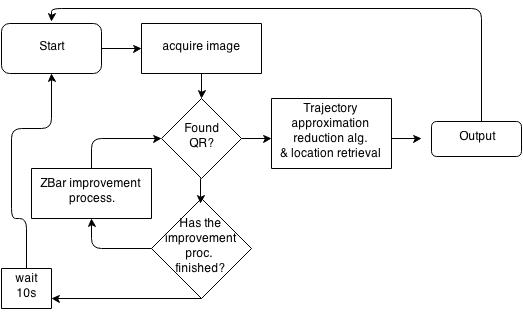
\includegraphics[scale=0.8]{img/workflow.jpg}
    \caption{The process main steps \label{workflow}}
\end{figure}

